% =========================================================================
%  ObelyZK: Verifiable Linear-Trace Inference for Billion-Parameter
%           Neural Networks via GKR Sumcheck with Aggregated Weight
%           Binding on Starknet
%
%  Target: arXiv cs.CR / cs.LG    |   Two-column, ~18 pages
%
%  License: CC BY 4.0
% =========================================================================
\documentclass[10pt,twocolumn]{article}

% ---------- packages ----------
\usepackage[utf8]{inputenc}
\usepackage[T1]{fontenc}
\usepackage{lmodern}
\usepackage[margin=0.75in]{geometry}
\usepackage{amsmath,amssymb,amsthm}
\usepackage{mathtools}
\usepackage{tikz}
\usetikzlibrary{arrows.meta,positioning,calc,decorations.pathreplacing,
                 fit,shapes.geometric,patterns,backgrounds}
\usepackage{pgfplots}
\pgfplotsset{compat=1.18}
\usepackage{booktabs}
\usepackage{tabularx}
\usepackage{multirow}
\usepackage{enumitem}
\usepackage{hyperref}
\usepackage{cleveref}
\usepackage{xcolor}
\usepackage{algorithm}
\usepackage{algpseudocode}
\usepackage{caption}
\usepackage{subcaption}
\usepackage[numbers,sort&compress]{natbib}
\usepackage{microtype}
\usepackage{url}
\usepackage{fancyhdr}
\usepackage{titlesec}
\usepackage{tcolorbox}
\usepackage{pifont}

% ---------- colours ----------
\definecolor{starkblue}{HTML}{2563eb}
\definecolor{accentpurple}{HTML}{7c3aed}
\definecolor{darkgray}{HTML}{333333}
\definecolor{emerald}{HTML}{059669}
\definecolor{warmred}{HTML}{dc2626}

% ---------- theorem environments ----------
\newtheorem{theorem}{Theorem}[section]
\newtheorem{lemma}[theorem]{Lemma}
\newtheorem{proposition}[theorem]{Proposition}
\newtheorem{corollary}[theorem]{Corollary}
\theoremstyle{definition}
\newtheorem{definition}[theorem]{Definition}
\newtheorem{protocol}[theorem]{Protocol}
\theoremstyle{remark}
\newtheorem{remark}[theorem]{Remark}

% ---------- macros ----------
\newcommand{\F}{\mathbb{F}}
\newcommand{\Fp}{\mathbb{F}_p}
\newcommand{\M}{\mathrm{M31}}
\newcommand{\CM}{\mathrm{CM31}}
\newcommand{\QM}{\mathrm{QM31}}
\newcommand{\eq}{\mathrm{eq}}
\newcommand{\MLE}{\widetilde}
\newcommand{\poly}{\mathrm{poly}}
\newcommand{\calP}{\mathcal{P}}
\newcommand{\calV}{\mathcal{V}}
\DeclareMathOperator{\loguptwo}{LogUp}
\DeclareMathOperator{\prhash}{Poseidon2}

% ---------- header / footer ----------
\pagestyle{fancy}
\fancyhf{}
\fancyhead[L]{\small\textit{ObelyZK: Verifiable Linear-Trace Inference via GKR}}
\fancyhead[R]{\small\thepage}
\renewcommand{\headrulewidth}{0.4pt}

% ---------- compact section titles ----------
\titlespacing*{\section}{0pt}{1.2ex plus 0.3ex minus 0.2ex}{0.6ex plus 0.1ex}
\titlespacing*{\subsection}{0pt}{0.8ex plus 0.2ex minus 0.1ex}{0.4ex plus 0.1ex}

% =========================================================================
\begin{document}

% ---- title ----
\makeatletter
\twocolumn[
\begin{@twocolumnfalse}
\begin{center}
  {\LARGE\bfseries ObelyZK: Verifiable Linear-Trace Inference for\par
   \vspace{4pt}
   Billion-Parameter Neural Networks via GKR Sumcheck\par
   \vspace{4pt}
   with Aggregated Weight Binding on Starknet}

  \vspace{12pt}

  {\large Victor Amaya, Bitsage Network}\par
  \vspace{4pt}
  {\small\texttt{info@obelysk.xyz}}

  \vspace{8pt}

  {\small March 2026}

  \vspace{10pt}

  \begin{minipage}{0.92\textwidth}
    \small\textbf{Abstract.}
    We present ObelyZK, a system that cryptographically verifies the
    \emph{linear arithmetic trace} of neural-network inference---matrix
    multiplications, additions, and scaling operations---for models up
    to 14 billion parameters, deployed on Starknet.
    The core contribution is \emph{aggregated weight binding}: a
    mismatch-sumcheck protocol that reduces the on-chain calldata
    required to verify 160 weight matrices from 2.4\,M~felts to
    86{,}723~felts ($\approx$28$\times$), making streaming
    verification of LLM-scale proofs practical within Starknet's
    per-transaction step limits.
    The system operates over the Mersenne prime field
    $p = 2^{31}-1$, extended through a degree-4 tower
    $\M \to \CM \to \QM$ providing 124-bit algebraic security,
    and achieves 3.04\,s per-layer GPU proving on NVIDIA H100.
    The on-chain Cairo verifier ({\raise.17ex\hbox{$\scriptstyle\sim$}}14\,K
    lines) accepts proofs via 18 streaming transactions and is
    deployed on Starknet Sepolia.
    We provide formal soundness analysis: at the recommended
    operational setting of $q=10$ MLE spot-check queries,
    the end-to-end forgery probability for the linear trace
    is bounded by $2^{-111}$ (conservatively; the MLE opening
    component alone achieves $2^{-130}$).
    \textbf{Scope:} The deployed verifier (v33) constrains
    linear operations, nonlinear activations
    via range-reduced LogUp (GELU, Sigmoid, Softmax verified
    on lower 16--20 bits; ReLU via algebraic proof), and
    the full Fiat-Shamir transcript via a 9-round-hardened
    replay verifier covering all 11 GKR layer tags,
    deferred proofs, and weight binding.
    LayerNorm/RMSNorm mean/variance remain unconstrained;
    we discuss the path to full inference verification.
  \end{minipage}

  \vspace{8pt}
  {\scriptsize\textbf{Keywords:}
    verifiable inference, linear arithmetic trace, GKR protocol,
    sumcheck, aggregated weight binding, STARK, Starknet, M31}

  \vspace{10pt}
\end{center}
\end{@twocolumnfalse}
]
\makeatother

% =========================================================================
\section{Introduction}\label{sec:intro}
% =========================================================================

Verifying that a specific neural network with committed weights produced a
specific output for a given input is a fundamental problem for AI
accountability, regulatory compliance, and trustless computation
markets~\cite{kang2022scaling, sun2024zkllm}.
Existing ZKML systems face a scalability wall:
EZKL~\cite{ezkl2024} handles $\sim$1\,M parameters via Halo2/KZG;
Giza~\cite{giza2024} uses Cairo-STARK for small models;
zkLLM~\cite{sun2024zkllm} demonstrates 13\,B-parameter proving but
requires 1--15 minutes and lacks a deployed on-chain verifier.

The central obstacle at LLM scale is \emph{on-chain calldata}:
a 40-layer transformer with 160 weight matrices requires
$\sim$2.4\,M field elements for individual MLE openings,
exceeding any L2's per-transaction limits.
This paper's main contribution addresses this bottleneck directly.

\subsection{Contributions}

\begin{enumerate}[nosep,leftmargin=1.4em]
  \item \textbf{Aggregated weight binding} (\Cref{sec:binding}) ---
        a mismatch-sumcheck protocol that batches 160 weight-matrix
        MLE openings into a single global oracle, reducing calldata
        from 2.4\,M to 86{,}723~felts ($\approx$28$\times$).
        This is the key enabler for on-chain LLM verification.
  \item \textbf{Cairo-native GKR streaming verifier}
        (\Cref{sec:onchain}) --- $\sim$14\,K lines of Cairo
        implementing the complete field tower, Fiat-Shamir channel,
        sumcheck, MLE opening, and aggregated binding verification
        across 18 streaming transactions.
        Contract v31, class hash
        \texttt{\small 0x6a6b\ldots5439}, deployed on Starknet Sepolia.
  \item \textbf{GPU-accelerated GKR proving}
        (\Cref{sec:gpu}) --- 3.04\,s per transformer layer for
        Qwen3-14B on NVIDIA H100, with 17+ custom CUDA kernels.
  \item \textbf{Formal security analysis} (\Cref{sec:security}) ---
        four theorems establishing soundness bounds for each
        verification component, with an explicit characterization of
        what the deployed verifier does and does not constrain.
\end{enumerate}

\subsection{Scope and Honest Assessment}

\Cref{tab:status} summarizes what is deployed, implemented, and
specified.
The deployed verifier (v33) cryptographically constrains
\emph{linear operations} (matmul, addition, scaling),
\emph{nonlinear activations} via range-reduced
LogUp~\cite{habock2022logup} (enforced by default), and
\emph{the full Fiat-Shamir transcript} via a replay verifier
covering all 11 GKR layer tags, deferred proofs, IO commitment,
and weight binding.
Activation inputs are masked to table range ($2^{16}$--$2^{20}$
entries) before proving; see \Cref{sec:limitations} for the
remaining gap (LayerNorm/RMSNorm mean/variance).

\begin{table}[t]
  \centering\scriptsize
  \caption{Implementation status matrix.
           \ding{51} = yes, \ding{55} = no, $\circ$ = partial.}
  \label{tab:status}
  \begin{tabular}{@{}lcccc@{}}
    \toprule
    \textbf{Component} & \textbf{Spec} & \textbf{Impl} & \textbf{Depl} & \textbf{Bench} \\
    \midrule
    MatMul sumcheck     & \ding{51} & \ding{51} & \ding{51} & \ding{51} \\
    Aggregated binding  & \ding{51} & \ding{51} & \ding{51} & \ding{51} \\
    Streaming verifier  & \ding{51} & \ding{51} & \ding{51} & \ding{51} \\
    MLE opening         & \ding{51} & \ding{51} & \ding{51} & \ding{51} \\
    Weight cache        & \ding{51} & \ding{51} & \ding{51} & \ding{51} \\
    Activation LogUp    & \ding{51} & \ding{51} & \ding{51} & $\circ$ \\
    Fiat-Shamir replay  & \ding{51} & \ding{51} & \ding{51} & --- \\
    Privacy layer       & \ding{51} & \ding{51} & \ding{51} & $\circ$ \\
    \bottomrule
  \end{tabular}

  \vspace{2pt}
  {\scriptsize Spec = protocol specified; Impl = code implemented;
   Depl = deployed on Starknet Sepolia; Bench = included in
   reported benchmarks.}
\end{table}

\subsection{Paper Organization}

\Cref{sec:prelim} presents the M31 field tower and MLE foundations.
\Cref{sec:gkr,sec:sumcheck} detail the GKR and sumcheck protocols.
\Cref{sec:binding} presents aggregated weight binding (the core
contribution).
\Cref{sec:gpu} discusses GPU acceleration.
\Cref{sec:onchain} details on-chain streaming verification.
\Cref{sec:security} provides a theorem-driven security analysis.
\Cref{sec:bench} reports benchmarks with a comparison to prior work.
\Cref{sec:limitations} discusses limitations and future work.
\Cref{sec:related} surveys related work.
\Cref{sec:conclusion} concludes.


% =========================================================================
\section{Preliminaries and Field Tower}\label{sec:prelim}
% =========================================================================

\subsection{The Mersenne Prime Field \texorpdfstring{$\M$}{M31}}

All arithmetic operates over $\Fp = \mathbb{Z}/p\mathbb{Z}$ with
$p = 2^{31}-1 = 2{,}147{,}483{,}647$.

\begin{lemma}[Efficient reduction]\label{lem:reduction}
  For $a,b \in \Fp$, let $w = a \cdot b$ as a 62-bit integer.
  Write $w = \mathit{lo} + \mathit{hi} \cdot 2^{31}$ where
  $\mathit{lo} = w \bmod 2^{31}$ and
  $\mathit{hi} = \lfloor w/2^{31}\rfloor$.
  Then
  \begin{equation}\label{eq:m31-reduce}
    a \cdot b \bmod p =
    \begin{cases}
      \mathit{lo} + \mathit{hi} & \text{if } \mathit{lo}+\mathit{hi} < p,\\
      \mathit{lo} + \mathit{hi} - p & \text{otherwise.}
    \end{cases}
  \end{equation}
\end{lemma}

\begin{proof}
  Since $p = 2^{31}-1$, we have $2^{31} \equiv 1 \pmod{p}$.
  Therefore $w = \mathit{lo} + \mathit{hi}\cdot 2^{31}
  \equiv \mathit{lo} + \mathit{hi} \pmod{p}$.
  Now $\mathit{lo} \in [0, 2^{31})$ and
  $\mathit{hi} \in [0, 2^{31})$ (since $w < p^2 < 2^{62}$),
  so $\mathit{lo}+\mathit{hi} \in [0, 2^{32}-2]$.
  Since $p = 2^{31}-1$, the sum can be at most $2p$, so at most
  one subtraction of~$p$ suffices to reduce to $[0,p)$.
\end{proof}

Field operations map directly to SIMD/GPU instructions:
\begin{itemize}[nosep,leftmargin=1.2em]
  \item \textbf{Addition:} $a+b$; subtract~$p$ if $\ge p$.
  \item \textbf{Multiplication:} 64-bit multiply, shift, mask, add,
        conditional subtract (\Cref{lem:reduction}).
  \item \textbf{Inversion:} $a^{p-2}\bmod p$ via Fermat's little theorem,
        using an addition chain of length 37.
\end{itemize}

\subsection{Field Extension Tower}

\begin{definition}[CM31 --- Complex Extension]
  $\CM = \M[i]/(i^2+1)$, elements $z = a+bi$ with $a,b \in \M$.
  The polynomial $x^2+1$ is irreducible since $-1$ is a quadratic
  non-residue mod~$p$ (because $p\equiv 3\pmod{4}$).
\end{definition}

\textbf{CM31 multiplication:}
$(a + bi)(c + di) = (ac - bd) + (ad + bc)i$.

\begin{definition}[QM31 --- the Secure Field]\label{def:qm31}
  $\QM = \CM[j]/(j^2-(2+i))$, elements $\alpha + \beta j$ with
  $\alpha,\beta \in \CM$.
  Each $\QM$ element has $4\times 31 = 124$ bits of algebraic security.
\end{definition}

\begin{lemma}[QM31 Karatsuba multiplication]\label{lem:qm31}
  For $x = \alpha_1 + \beta_1 j$ and $y = \alpha_2 + \beta_2 j$ in $\QM$:
  \begin{multline}\label{eq:qm31-mul}
    x \cdot y = \bigl(\alpha_1\alpha_2 + \beta_1\beta_2\cdot u\bigr) \\
    + \bigl((\alpha_1\!+\!\beta_1)(\alpha_2\!+\!\beta_2)
    - \alpha_1\alpha_2 - \beta_1\beta_2\bigr)j,
  \end{multline}
  where $u = 2+i$ is the irreducible element and the multiplication
  by~$u$ in $\CM$ is: $(a+bi)\cdot(2+i) = (2a-b) + (a+2b)i$.
\end{lemma}

\begin{proof}
  Expanding $({\alpha_1+\beta_1 j})({\alpha_2+\beta_2 j})$ and
  using $j^2 = 2+i = u$ gives the real part
  $\alpha_1\alpha_2 + \beta_1\beta_2\,u$ and cross term
  $\alpha_1\beta_2 + \beta_1\alpha_2$.
  The Karatsuba identity
  $\alpha_1\beta_2+\beta_1\alpha_2 = (\alpha_1+\beta_1)(\alpha_2+\beta_2)-\alpha_1\alpha_2-\beta_1\beta_2$
  reduces from 4 to 3 CM31 multiplications.
\end{proof}

% ---------- TikZ: Field Tower ----------
\begin{figure}[t]
  \centering
  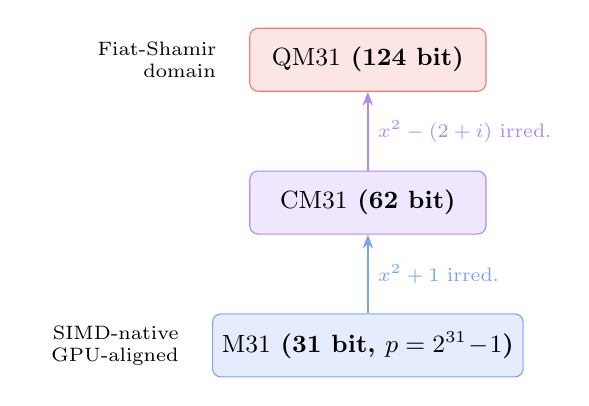
\begin{tikzpicture}[
    box/.style={draw, rounded corners=3pt, minimum width=3cm,
                minimum height=0.8cm, font=\small\bfseries,
                fill=#1!12, draw=#1!60},
    arr/.style={-{Stealth[length=5pt]}, thick, #1!60},
    node distance=1cm
  ]
    \node[box=starkblue] (m31) {$\M$ \small(31 bit, $p=2^{31}\!-\!1$)};
    \node[box=accentpurple, above=of m31] (cm31) {$\CM$ \small(62 bit)};
    \node[box=warmred, above=of cm31] (qm31) {$\QM$ \small(124 bit)};

    \draw[arr=starkblue]  (m31)  -- node[right,font=\scriptsize]{$x^2+1$ irred.} (cm31);
    \draw[arr=accentpurple] (cm31) -- node[right,font=\scriptsize]{$x^2-(2+i)$ irred.} (qm31);

    % Annotations
    \node[font=\scriptsize, left=0.3cm of m31, text width=1.8cm, align=right]
      {SIMD-native\\GPU-aligned};
    \node[font=\scriptsize, left=0.3cm of qm31, text width=1.8cm, align=right]
      {Fiat-Shamir\\domain};
  \end{tikzpicture}
  \caption{M31 field extension tower. The base field enables hardware-efficient
           arithmetic; the quartic extension provides 124-bit security for
           the Fiat-Shamir channel.}
  \label{fig:tower}
\end{figure}

\subsection{Multilinear Extensions (MLEs)}

\begin{definition}[Multilinear extension]
For $f:\{0,1\}^n\to\F$, the unique multilinear polynomial agreeing
with~$f$ on the Boolean hypercube is:
\begin{equation}\label{eq:mle}
  \MLE{f}(x_1,\ldots,x_n)
  = \sum_{y\in\{0,1\}^n} f(y)\prod_{i=1}^{n}
    \bigl(x_i y_i + (1\!-\!x_i)(1\!-\!y_i)\bigr).
\end{equation}
\end{definition}

The \emph{Lagrange equality kernel} is
$\eq(\mathbf{x},\mathbf{y}) = \prod_{i=1}^n (x_i y_i + (1-x_i)(1-y_i))$,
evaluating to~1 when $\mathbf{x}=\mathbf{y}$ on the Boolean hypercube.

\textbf{MLE folding.}
Fixing variable $x_1=r$ reduces the MLE dimension by one:
\begin{equation}\label{eq:fold}
  \MLE{f}|_{x_1=r}(x_2,\ldots,x_n)
  = (1-r)\cdot\MLE{f}(0,x_2,\ldots) + r\cdot\MLE{f}(1,x_2,\ldots).
\end{equation}
This operation is linear in the table size and is the core primitive
for both the sumcheck prover and the MLE opening verifier.


% =========================================================================
\section{GKR for Neural Networks}\label{sec:gkr}
% =========================================================================

\subsection{Protocol Overview}

The GKR protocol~\cite{goldwasser2015delegating, thaler2013time} verifies
layered arithmetic circuits by reducing an output claim to an input
claim one layer at a time.
For a neural network with $L$ layers:
\[
  \text{Input} \xrightarrow{\text{Layer 1}} h_1
  \xrightarrow{\text{Layer 2}} h_2
  \xrightarrow{\;\cdots\;}
  h_{L-1} \xrightarrow{\text{Layer }L} \text{Output}.
\]
The verifier starts with a claim about the output and reduces it
backward through each layer via the sumcheck
protocol~\cite{lund1992algebraic}.
Per-layer verification cost is $O(\log n)$ for layer width~$n$,
regardless of the actual computation size.

% ---------- TikZ: GKR Reduction ----------
\begin{figure}[t]
  \centering
  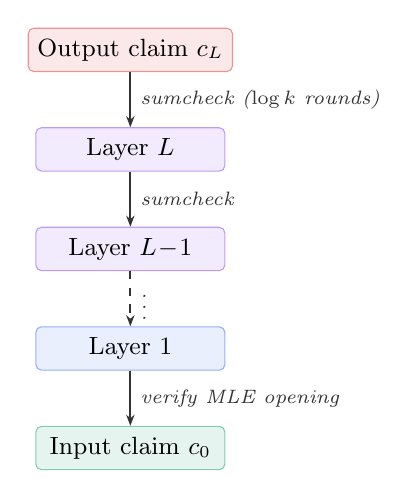
\begin{tikzpicture}[
    layer/.style={draw, rounded corners=2pt, minimum width=2.4cm,
                  minimum height=0.55cm, font=\small, fill=#1!10, draw=#1!50},
    arr/.style={-{Stealth[length=4pt]}, thick, darkgray},
    clbl/.style={font=\scriptsize\itshape, darkgray}
  ]
    \node[layer=warmred]          (out) {Output claim $c_L$};
    \node[layer=accentpurple, below=0.7cm of out] (l3)  {Layer $L$};
    \node[layer=accentpurple, below=0.7cm of l3]  (l2)  {Layer $L\!-\!1$};
    \node[layer=starkblue,    below=0.7cm of l2]  (l1)  {Layer 1};
    \node[layer=emerald,      below=0.7cm of l1]  (inp) {Input claim $c_0$};

    \draw[arr] (out) -- node[right,clbl]{sumcheck ($\log k$ rounds)} (l3);
    \draw[arr] (l3)  -- node[right,clbl]{sumcheck} (l2);
    \draw[arr,dashed] (l2) -- node[right,clbl]{$\vdots$} (l1);
    \draw[arr] (l1)  -- node[right,clbl]{verify MLE opening} (inp);
  \end{tikzpicture}
  \caption{GKR claim reduction: each layer reduces an output claim to an
           input claim via sumcheck. After $L$ reductions, the verifier
           checks the final claim against the committed input MLE.}
  \label{fig:gkr-reduction}
\end{figure}

\subsection{Layer Types}

\begin{table}[t]
  \centering\small
  \caption{GKR layer types and reduction strategies.
           All 11 layer tags are constrained in the deployed verifier (v33).}
  \label{tab:layers}
  \begin{tabularx}{\columnwidth}{@{}lcccX@{}}
    \toprule
    \textbf{Layer} & \textbf{Tag} & \textbf{Deg.} & \textbf{Rnds} & \textbf{Strategy} \\
    \midrule
    MatMul$(m,k,n)$     & 0 & 2 & $\log_2 k$ & Product of two MLEs \\
    Add$(n)$            & 1 & 1 & 1          & Linearity: $c_0=\text{claim}/2$ \\
    Mul$(n)$            & 2 & 2 & 1          & Degree-2 check \\
    Activation          & 3 & 3 & $\log_2 n$ & LogUp (GELU/Sigmoid/Softmax) or algebraic (ReLU) \\
    LayerNorm           & 4 & 3 & $\log_2 n$ & Linear eq-sum + rsqrt LogUp \\
    GQA Attention       & 5 & 2 & decomposed & Q$\times$K, $\times$V sub-proofs \\
    Dequantize          & 6 & 3 & $\log_2 n$ & Range-reduced LogUp \\
    MatMulDualSimd      & 7 & 3 & $\log_2 k$ & Block-partitioned degree-3 \\
    RMSNorm             & 8 & 3 & $\log_2 n$ & Linear eq-sum + rsqrt LogUp \\
    Quantize            & 9 & 3 & $\log_2 n$ & Range-reduced LogUp \\
    Embedding           & 10 & 3 & $\log_2 n$ & Sparse table LogUp \\
    \bottomrule
  \end{tabularx}
\end{table}

The GKR circuit supports 11 layer tags (\Cref{tab:layers}),
including quantization/dequantization layers with metadata-keyed
LogUp and embedding layers with sparse-table lookups.

Self-attention with Grouped Query Attention
(GQA) computes:
\[
  \text{Attention}(Q,K,V)
  = \text{softmax}\!\left(\frac{QK^T}{\sqrt{d_k}}\right)\!V
\]
We decompose this into five sublayers: QK$^T$ matmul (degree~2),
scaling (degree~1), causal mask (linear), softmax (range-reduced LogUp),
and score$\times$V matmul (degree~2).
RoPE encoding is a linear layer with position-dependent trigonometric
coefficients precomputed as an MLE.

\subsection{Batch Verification}

Multiple layer instances $\{I_1,\ldots,I_m\}$ with claims
$\{c_1,\ldots,c_m\}$ are batched via random linear combination.
The verifier draws $\alpha,\lambda\leftarrow\QM$ from the Fiat-Shamir
channel and forms the batched claim:
\begin{equation}\label{eq:batch}
  S = \sum_{i=1}^{m} \alpha^i \cdot 2^{n_{\max}-n_i} \cdot
  \biggl(\sum_j \lambda^j \cdot c_{i,j}\biggr),
\end{equation}
where $n_{\max}-n_i$ is the padding doubling factor for instance~$i$.

\subsection{Fiat-Shamir Channel}

The interactive protocol is made non-interactive via a Poseidon252-based
Fiat-Shamir channel~\cite{fiat1986prove}:
\begin{itemize}[nosep,leftmargin=1.2em]
  \item State: $(\text{digest}: \text{felt252},\; n\_\text{draws}: \text{u32})$.
  \item \texttt{mix\_felt(v)}: $\text{digest} \leftarrow
        \text{Hades}(\text{digest}, v, 2)[0]$; $n\_\text{draws}\leftarrow 0$.
  \item \texttt{draw\_qm31()}: draw felt252, extract 4 M31 components
        via successive $\bmod\,2^{31}$.
\end{itemize}


% =========================================================================
\section{Sumcheck for Matrix Multiplication}\label{sec:sumcheck}
% =========================================================================

\subsection{Problem Formulation}

Given $A\in\F^{m\times k}$, $B\in\F^{k\times n}$, claimed $C=AB$,
and random evaluation points $\mathbf{r}_i\in\F^{\log m}$,
$\mathbf{r}_j\in\F^{\log n}$:
\begin{equation}\label{eq:matmul-sumcheck}
  \MLE{C}(\mathbf{r}_i,\mathbf{r}_j)
  = \sum_{\mathbf{x}\in\{0,1\}^{\log k}}
    \MLE{A}(\mathbf{r}_i,\mathbf{x})\cdot\MLE{B}(\mathbf{x},\mathbf{r}_j).
\end{equation}
This is a sum over $k$ terms of a degree-2 polynomial (product of two
MLEs), exactly the form required by the sumcheck protocol.

\textbf{MLE layout.}
Matrix~$A$ uses row-major layout; matrix~$B$ uses column-major
(transposed) layout, enabling fixing the $k$-dimension variables first.

\subsection{Round Protocol}

\begin{algorithm}[t]
\caption{Sumcheck round for MatMul verification}
\label{alg:sumcheck}
\begin{algorithmic}[1]
\Require MLEs $f_a, f_b$ of length $2\cdot\mathrm{mid}$; current claim
\State $S_0 \leftarrow \sum_{i=0}^{\mathrm{mid}-1} f_a[i] \cdot f_b[i]$
\State $S_1 \leftarrow \sum_{i=0}^{\mathrm{mid}-1}
  f_a[\mathrm{mid}+i] \cdot f_b[\mathrm{mid}+i]$
\State $S_2 \leftarrow \sum_{i=0}^{\mathrm{mid}-1}
  (2f_a[\mathrm{mid}+i] - f_a[i])
  (2f_b[\mathrm{mid}+i] - f_b[i])$
\State Lagrange interpolate: $p(X) = c_0 + c_1 X + c_2 X^2$
\State \textbf{assert} $c_0 + (c_0+c_1+c_2) = \text{claim}$
  \Comment{$p(0)+p(1)$}
\State Send $(c_0, c_2)$; verifier reconstructs
  $c_1 = \text{claim} - 2c_0 - c_2$
\State $r_t \leftarrow$ Fiat-Shamir challenge
\State Fold: $f_a^{(t+1)}[i] = f_a[i] + r_t\,(f_a[\mathrm{mid}+i]-f_a[i])$
\State Update claim: $p(r_t) = c_0 + r_t(c_1 + r_t\,c_2)$ (Horner)
\end{algorithmic}
\end{algorithm}

\textbf{Proof compression.}
Only $(c_0,c_2)$ are transmitted per round; the verifier reconstructs
$c_1 = \text{claim} - 2c_0 - c_2$, saving 33\% of calldata.


% =========================================================================
\section{Aggregated Weight Binding}\label{sec:binding}
% =========================================================================

This section presents the paper's core contribution: a protocol that
makes on-chain verification of LLM-scale weight commitments practical.

\subsection{The Calldata Bottleneck}

A 40-layer Qwen3-14B has 160 weight matrices.
Verifying each independently requires an MLE opening proof per matrix,
totaling $\sim$2.4\,M felts of calldata.
Starknet's per-transaction step limit ($\sim$10\,M Cairo steps) makes
processing this volume infeasible in streaming transactions.

\subsection{Global Oracle Construction}

\begin{definition}[Global weight oracle]\label{def:global-oracle}
  Given $M$ weight matrices $\{W_1,\ldots,W_M\}$ with dimensions
  $\{(r_i,c_i)\}_{i=1}^M$, the global oracle MLE is:
  \begin{equation}\label{eq:global}
    W_{\text{global}}(\mathbf{s},\mathbf{x})
    = \sum_{i=1}^{M} \eq(\mathbf{s},\mathbf{g}_i)
      \cdot \MLE{W_i}(\mathbf{x}),
  \end{equation}
  where $\mathbf{s}\in\{0,1\}^{\lceil\log_2 M\rceil}$ are selector bits
  and $\mathbf{g}_i$ is the binary encoding of matrix index~$i$.
\end{definition}

\subsection{Mismatch Sumcheck Protocol}

\begin{protocol}[Aggregated weight binding]\label{prot:binding}
  Given $M$ weight matrices with claimed evaluations $v_i$ at
  points $\mathbf{e}_i$ (produced by the GKR sumcheck):
  \begin{enumerate}[nosep,leftmargin=1.4em]
    \item \textbf{Batch.} Draw $\rho\leftarrow\QM$ from the
          Fiat-Shamir channel.
    \item \textbf{Mismatch sumcheck.} Prove that the random
          linear combination of all mismatches vanishes:
      \begin{equation}\label{eq:binding}
        \sum_{i=1}^{M} \rho^i \cdot \eq(\mathbf{g}_i,\mathbf{s})
        \cdot \bigl(W_{\text{global}}(\mathbf{s},\mathbf{e}_i) - v_i\bigr) \equiv 0.
      \end{equation}
    \item \textbf{Commitment check.} Verify the final MLE opening
          against the committed Poseidon2-M31 super-root
          with subtree Merkle openings.
  \end{enumerate}
\end{protocol}

\textbf{Intuition.}
If all claimed evaluations are correct
($W_{\text{global}}(\mathbf{s},\mathbf{e}_i) = v_i$ for all~$i$),
every term in the sum is zero.
A cheating prover who forges even one evaluation $v_j$ must
produce a non-zero polynomial that sums to zero---which
by Schwartz-Zippel~\cite{schwartz1980,zippel1979} occurs with
probability at most $1/|\QM|\approx 2^{-124}$.

% ---------- TikZ: Aggregated Binding Concept ----------
\begin{figure}[t]
  \centering
  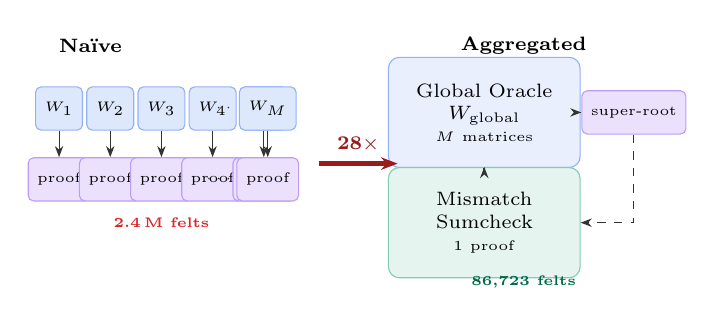
\begin{tikzpicture}[
    mat/.style={draw, rounded corners=2pt, minimum width=0.55cm,
                minimum height=0.55cm, font=\tiny, fill=#1!15, draw=#1!50},
    bigbox/.style={draw, rounded corners=4pt, minimum height=1.4cm,
                   text width=2.2cm, align=center, font=\scriptsize,
                   fill=#1!10, draw=#1!50},
    arr/.style={-{Stealth[length=4pt]}, thick, darkgray},
    lbl/.style={font=\tiny, darkgray},
    node distance=0.15cm
  ]
    % --- Left: Naive ---
    \node[font=\scriptsize\bfseries] at (-1.8,2) {Na\"ive};

    \foreach \i in {0,...,4} {
      \node[mat=starkblue] (w\i) at (-2.2+\i*0.65, 1.2) {$W_{\the\numexpr\i+1}$};
      \node[mat=accentpurple] (p\i) at (-2.2+\i*0.65, 0.3) {\tiny proof};
      \draw[arr, thin] (w\i) -- (p\i);
    }
    \node[font=\tiny, darkgray] at (-0.15,1.2) {$\cdots$};
    \node[font=\tiny, darkgray] at (-0.15,0.3) {$\cdots$};
    \node[mat=starkblue] (wn) at (0.45, 1.2) {$W_M$};
    \node[mat=accentpurple] (pn) at (0.45, 0.3) {\tiny proof};
    \draw[arr, thin] (wn) -- (pn);

    \node[font=\tiny\bfseries, warmred] at (-0.9, -0.25) {2.4\,M felts};

    % --- Right: Aggregated ---
    \node[font=\scriptsize\bfseries] at (3.7,2) {Aggregated};

    \node[bigbox=starkblue] (global) at (3.2, 1.15) {Global Oracle\\$W_{\text{global}}$\\{\tiny $M$ matrices}};
    \node[bigbox=emerald] (sc) at (3.2, -0.25) {Mismatch\\Sumcheck\\{\tiny 1 proof}};
    \draw[arr] (global) -- (sc);

    \node[mat=accentpurple, minimum width=1.2cm] (root) at (5.1, 1.15) {\tiny super-root};
    \draw[arr, thin] (global) -- (root);
    \draw[arr, thin, dashed] (root) |- (sc);

    \node[font=\tiny\bfseries, emerald!70!black] at (3.7, -1.0) {86{,}723 felts};

    % --- Arrow between ---
    \draw[-{Stealth[length=6pt]}, ultra thick, warmred!70!black]
      (1.1, 0.5) -- node[above, font=\scriptsize\bfseries]{28$\times$} (2.1, 0.5);
  \end{tikzpicture}
  \caption{Aggregated weight binding eliminates per-matrix opening
           proofs. Left: na\"ive approach requires one MLE opening per
           weight matrix ($\sim$2.4\,M felts). Right: a single global
           oracle with mismatch sumcheck verifies all 160 matrices
           (86{,}723 felts), a 28$\times$ reduction.}
  \label{fig:binding-concept}
\end{figure}

\subsection{Zero-Tree Commitment Extension}

Matrices with different depths are padded to $n_{\max}$ using
zero-tree hashing: $h_0 = \text{pack}(\QM::0)$,
$h_i = \text{poseidon\_hash}(h_{i-1}, h_{i-1})$.
This allows a single Merkle super-root to cover all weight matrices
regardless of individual dimensions.

\subsection{Streaming Calldata Breakdown}

\begin{table}[t]
  \centering\small
  \caption{Calldata for Qwen3-14B 40-layer proof.
           Aggregated binding reduces total calldata by 28$\times$.}
  \label{tab:calldata}
  \begin{tabular}{@{}lrr@{}}
    \toprule
    \textbf{Method} & \textbf{Felts} & \textbf{Bytes} \\
    \midrule
    Individual openings & $\sim$2{,}400{,}000 & $\sim$76.8\,MB \\
    Aggregated binding  & 86{,}723 & $\sim$2.8\,MB \\
    \quad GKR layer data & $\sim$82{,}433 & $\sim$2.6\,MB \\
    \quad Binding proof  & $\sim$4{,}290 & $\sim$137\,KB \\
    \midrule
    \textbf{Reduction}  & \multicolumn{2}{c}{\textbf{$\approx$28$\times$}} \\
    \bottomrule
  \end{tabular}
\end{table}

\subsection{Memory-Efficient Proving}

The off-chain binding prover uses \texttt{GraphWeightSource}---a
streaming interface that loads weight matrices on demand from the
model graph rather than materializing all 160 matrices simultaneously.
This bounds peak memory at $\sim$4\,GB (one weight matrix at a time)
versus $\sim$640\,GB for full materialization.

\subsection{Weight Commitment Cache}

Poseidon2-M31 Merkle root computation for 160 matrices takes
$\sim$500\,s on first run.
The weight cache (\texttt{.swcf} file) stores roots keyed by
$(node\_id, rows\_padded, cols\_padded)$, reducing subsequent
proofs to $<$1\,ms (cache hit) for the commitment phase.


% =========================================================================
\section{GPU-Accelerated Proving}\label{sec:gpu}
% =========================================================================

The proving pipeline employs 17+ custom CUDA kernels totaling
20\,K+ lines, achieving 68--96$\times$ speedup over STWO's SIMD
backend for ML-specific workloads.

\textbf{Sumcheck kernel.}
Block size 256, shared memory 12\,KB/block, dispatch threshold
$k\ge 2^{14}$.
Per-thread: load $(f_a[i], f_a[\text{mid}+i], f_b[i], f_b[\text{mid}+i])$,
compute partial $S_0, S_1, S_2$, then 8-iteration binary tree
reduction with \texttt{\_\_syncthreads()}.

\textbf{MLE fold kernel.}
512 threads/block, grid $= \lceil n/(2\cdot 512)\rceil$.
Output $[i] = f[i] + r\cdot(f[\text{mid}+i]-f[i])$ with challenge
broadcast (16 bytes).

\textbf{GPU M31 arithmetic.}
\begin{align*}
  \texttt{m31\_mul}(a,b) &: \text{prod} = (\text{u64})\,a\cdot b; \\
  &\quad \text{lo} = \text{prod}\;\&\;\texttt{0x7FFFFFFF}; \\
  &\quad \text{hi} = \text{prod}\gg 31; \\
  &\quad \textbf{return}\;\texttt{m31\_add}(\text{lo},\text{hi}).
\end{align*}

% ---------- pgfplots: GPU Speedup Bar Chart ----------
\begin{figure}[t]
  \centering
  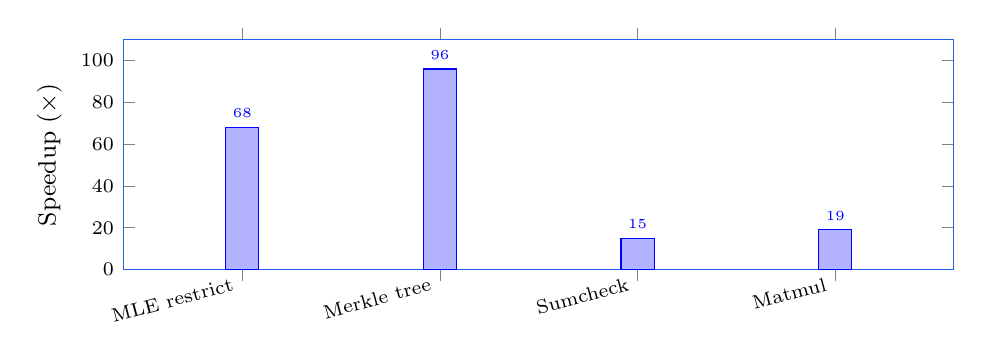
\begin{tikzpicture}
    \begin{axis}[
      ybar,
      bar width=12pt,
      width=\columnwidth,
      height=4.5cm,
      symbolic x coords={MLE restrict, Merkle tree, Sumcheck, Matmul},
      xtick=data,
      xticklabel style={font=\scriptsize, rotate=15, anchor=east},
      ylabel={Speedup ($\times$)},
      ylabel style={font=\small},
      ymin=0, ymax=110,
      ytick={0,20,40,60,80,100},
      yticklabel style={font=\scriptsize},
      nodes near coords,
      every node near coord/.append style={font=\tiny\bfseries},
      fill=starkblue!70,
      draw=starkblue,
      enlarge x limits=0.2,
    ]
    \addplot coordinates {
      (MLE restrict, 68)
      (Merkle tree, 96)
      (Sumcheck, 15)
      (Matmul, 19)
    };
    \end{axis}
  \end{tikzpicture}
  \caption{GPU (CUDA) speedup over CPU (STWO SIMD) for key operations
           on NVIDIA H100.}
  \label{fig:gpu-speedup}
\end{figure}

\textbf{Multi-GPU support.}
Weight commitment computation supports multi-GPU via greedy
bin-packing (\texttt{multi\_gpu::partition\_by\_size()}), with one
\texttt{DeviceGuard} per thread and fallback to single-GPU pipelined
path on failure.


% =========================================================================
\section{On-Chain Streaming Verification}\label{sec:onchain}
% =========================================================================

\subsection{Cairo Verifier Architecture}

The on-chain verifier (v33) comprises $\sim$14\,K lines of Cairo across
21~modules.
A Rust-side \emph{replay verifier} independently re-derives the
Fiat-Shamir channel state from serialized proof data before
submission, catching prover/serializer mismatches pre-flight
(\Cref{thm:deployed}, item~(f)).
Class hash:\par
{\small\texttt{0x6a6b...d5ec1f63d715...ffbaf6c5b5439}}.

\begin{table}[t]
  \centering\small
  \caption{Key Cairo verifier modules.}
  \label{tab:cairo}
  \begin{tabular}{@{}lr@{}}
    \toprule
    \textbf{Module} & \textbf{LOC} \\
    \midrule
    \texttt{aggregated\_binding.cairo} & 995 \\
    \texttt{gkr.cairo} & 547 \\
    \texttt{field.cairo} & 503 \\
    \texttt{types.cairo} & 367 \\
    \texttt{sumcheck.cairo} & 269 \\
    \texttt{mle.cairo} & 250+ \\
    \texttt{channel.cairo} & 244 \\
    \bottomrule
  \end{tabular}
\end{table}

\subsection{MLE Opening Verification}

\begin{enumerate}[nosep,leftmargin=1.4em]
  \item Commitment: $2^n$ evaluations $\to$ Poseidon2-M31 Merkle root.
  \item Folding: $n$ rounds, challenge $r_i$ per round:
    $f_{i+1}[j] = f_i[j] + r_i(f_i[\mathrm{mid}+j]-f_i[j])$.
  \item Spot checks: $q$ queries per fold (read from
    proof at runtime; default 5 via \texttt{MLE\_NUM\_QUERIES},
    recommended $q=10$ for production; see \Cref{thm:mle}).
  \item Verify Merkle paths and folding consistency at each layer.
\end{enumerate}

\subsection{18-Transaction Streaming Protocol}

% ---------- TikZ: End-to-End Proof Flow ----------
\begin{figure*}[t]
  \centering
  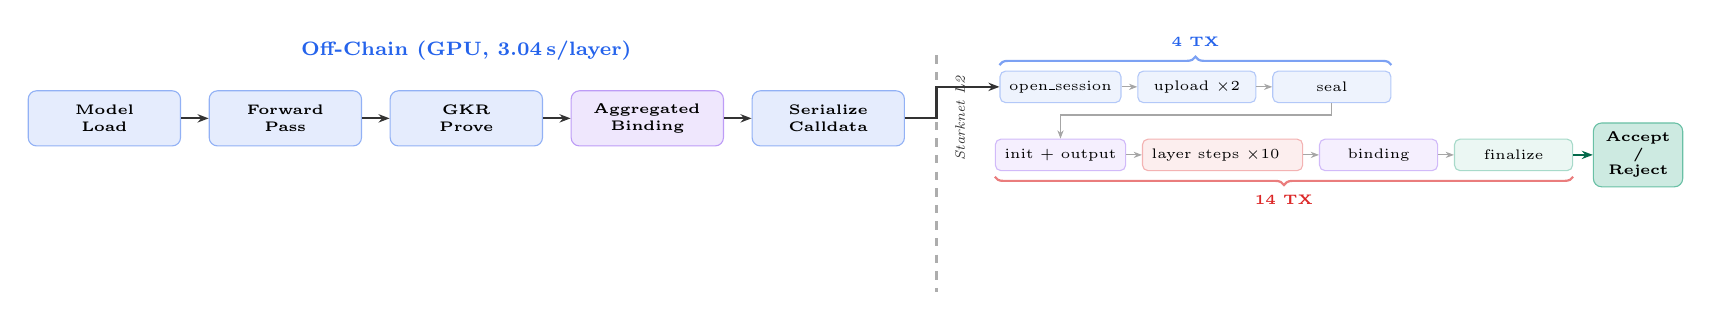
\begin{tikzpicture}[
    phase/.style={draw, rounded corners=3pt, minimum height=0.7cm,
                  text width=1.7cm, align=center, font=\tiny\bfseries,
                  fill=#1!12, draw=#1!50},
    step/.style={draw, rounded corners=2pt, minimum height=0.4cm,
                 minimum width=1.5cm, font=\tiny,
                 fill=#1!8, draw=#1!35},
    arr/.style={-{Stealth[length=4pt]}, thick, darkgray},
    sarr/.style={-{Stealth[length=3pt]}, thin, gray!70},
    lbl/.style={font=\tiny, darkgray},
    node distance=0.3cm and 0.35cm
  ]
    % === Off-chain ===
    \node[phase=starkblue] (load) {Model\\Load};
    \node[phase=starkblue, right=of load] (fwd) {Forward\\Pass};
    \node[phase=starkblue, right=of fwd] (gkr) {GKR\\Prove};
    \node[phase=accentpurple, right=of gkr] (bind) {Aggregated\\Binding};
    \node[phase=starkblue, right=of bind] (serial) {Serialize\\Calldata};

    \draw[arr] (load) -- (fwd);
    \draw[arr] (fwd) -- (gkr);
    \draw[arr] (gkr) -- (bind);
    \draw[arr] (bind) -- (serial);

    \node[font=\scriptsize\bfseries, starkblue, above=0.25cm of gkr]
      {Off-Chain (GPU, 3.04\,s/layer)};

    % === Boundary ===
    \draw[dashed, thick, darkgray!40]
      ([xshift=0.4cm]serial.east) ++(0,0.8) -- ++(0,-3.0);
    \node[font=\tiny\itshape, darkgray, rotate=90]
      at ([xshift=0.7cm]serial.east) {Starknet L2};

    % === On-chain: Session ===
    \node[step=starkblue, right=1.2cm of serial, yshift=0.4cm]
      (tx1) {open\_session};
    \node[step=starkblue, right=0.2cm of tx1]
      (tx2) {upload $\times$2};
    \node[step=starkblue, right=0.2cm of tx2]
      (tx3) {seal};

    \draw[sarr] (tx1) -- (tx2);
    \draw[sarr] (tx2) -- (tx3);
    \draw[arr] (serial.east) -- ++(0.4,0) |- (tx1.west);

    % === On-chain: Verification ===
    \node[step=accentpurple, below=0.45cm of tx1]
      (v1) {init + output};
    \node[step=warmred, right=0.2cm of v1, text width=1.8cm]
      (v2) {layer steps $\times$10};
    \node[step=accentpurple, right=0.2cm of v2]
      (v3) {binding};
    \node[step=emerald, right=0.2cm of v3]
      (v4) {finalize};

    \draw[sarr] (tx3.south) -- ++(0,-0.15) -| (v1.north);
    \draw[sarr] (v1) -- (v2);
    \draw[sarr] (v2) -- (v3);
    \draw[sarr] (v3) -- (v4);

    % Verdict
    \node[draw, rounded corners=3pt, fill=emerald!20, draw=emerald!60,
          font=\tiny\bfseries, right=0.25cm of v4, minimum height=0.5cm,
          text width=0.9cm, align=center]
      (verdict) {Accept /\\ Reject};
    \draw[arr, emerald!70!black] (v4) -- (verdict);

    % Braces
    \draw[decorate, decoration={brace,amplitude=3pt},
          thick, starkblue!60]
      ([yshift=2pt]tx1.north west) -- ([yshift=2pt]tx3.north east)
      node[midway, above=3pt, font=\tiny\bfseries, starkblue]{4 TX};
    \draw[decorate, decoration={brace,amplitude=3pt,mirror},
          thick, warmred!60]
      ([yshift=-2pt]v1.south west) -- ([yshift=-2pt]v4.south east)
      node[midway, below=3pt, font=\tiny\bfseries, warmred]{14 TX};
  \end{tikzpicture}
  \caption{End-to-end proof flow. Off-chain: model loading, M31 forward
           pass, GKR proving, aggregated binding, and calldata serialization.
           On-chain: 18 Starknet transactions split into 4 session management
           and 14 streaming verification steps, ending with an accept/reject
           verdict.}
  \label{fig:streaming}
\end{figure*}

The streaming protocol (\Cref{fig:streaming}) splits verification
across 18 transactions to fit within Starknet's per-TX step limit:
\begin{enumerate}[nosep,leftmargin=1.4em]
  \item \textbf{Session phase} (TXs 1--4): open session, upload
        calldata in chunks, seal session.
  \item \textbf{Verification phase} (TXs 5--18): init channel state,
        verify output MLE, process 10 layer steps (each running
        sumcheck verification), verify aggregated weight binding,
        finalize with input MLE check and verdict.
\end{enumerate}

\textbf{QM31 packing.}
QM31 values are packed into felt252:
$\text{packed} = 1\cdot 2^{124} + a_0\cdot 2^{93} + a_1\cdot 2^{62}
+ b_0\cdot 2^{31} + b_1$
(125 bits used, 1-bit sentinel prevents zero ambiguity).

\textbf{IO-packed calldata.}
8 M31 per felt252, reducing IO calldata from 10{,}246 to 1{,}281 felts.
\texttt{evaluate\_mle\_from\_packed\_1row()} evaluates the MLE directly
from packed felts without unpacking.


% =========================================================================
\section{Security Analysis}\label{sec:security}
% =========================================================================

We present four theorems establishing the soundness of each
verification component. All security statements are in the
random oracle model for Fiat-Shamir.

\subsection{Threat Model}

We consider a computationally unbounded malicious prover $\calP^*$
attempting to convince the on-chain verifier $\calV$ to accept an
incorrect result.
Assumptions:
\begin{itemize}[nosep,leftmargin=1.2em]
  \item The Fiat-Shamir hash (Poseidon252) is modeled as a random
        oracle binding transcript challenges to the full history.
  \item Starknet L2 provides data availability and transaction
        ordering guarantees.
  \item The prover must produce a valid transcript accepted by the
        Cairo verifier contract; no physical access to the verifier
        is assumed.
\end{itemize}

\subsection{Theorem 1: Sumcheck Soundness Per Layer}

\begin{theorem}[Sumcheck soundness]\label{thm:sumcheck}
  For a degree-$d$ sumcheck polynomial over $\QM$ with $k$ rounds,
  a cheating prover passes with probability at most
  $kd/|\QM|$~\cite{lund1992algebraic, schwartz1980, zippel1979}.
  For matmul with $k=\lceil\log_2 5120\rceil = 13$ and $d=2$:
  \[
    \varepsilon_{\text{sc}} \le \frac{13\times 2}{2^{124}}
    = \frac{26}{2^{124}} \approx 2^{-119}.
  \]
\end{theorem}

\begin{proof}
  Each sumcheck round requires the prover to send a degree-$d$
  univariate polynomial $p_i(X)$ such that $p_i(0)+p_i(1)$ equals
  the current claim.
  By Schwartz-Zippel, a dishonest $p_i$ agrees with the honest
  polynomial at the random challenge $r_i$ with probability at
  most $d/|\QM|$.
  By union bound over $k$ rounds, the total cheating probability
  is at most $kd/|\QM|$.
\end{proof}

\subsection{Theorem 2: MLE Opening Soundness}

\begin{theorem}[MLE opening soundness]\label{thm:mle}
  Consider the MLE opening protocol with $n$ folds and $q$
  spot-check queries per fold, where queries are sampled
  uniformly without replacement from the folded table at each
  round.
  At fold~$i$, the table has $2^{n-i}$ entries and $q$ positions
  are checked.
  A cheating prover who substitutes an incorrect folded value at
  any position must avoid all $q$ checks at that fold.
  Under the assumption that the Fiat-Shamir transcript
  (which determines query positions) behaves as a random oracle,
  the probability of evading detection at a single fold is:
  \[
    \Pr[\text{evade fold } i] \le 1 - \frac{q}{2^{n-i}}.
  \]
  Since $2^{n-i} \ge 2$ for all folds ($i < n$), this gives
  $\Pr[\text{evade}] \le 1 - q/2^{n-i} \le (1-1/2)^q = 2^{-q}$
  as a conservative per-fold bound (worst case at the final fold
  where the table has only 2 entries).

  The total evasion probability over $n$ folds is then
  conservatively bounded by:
  \begin{equation}\label{eq:mle-sound}
    \varepsilon_{\text{mle}} \le 2^{-qn}.
  \end{equation}

  For $n=13$ folds:
  \begin{itemize}[nosep,leftmargin=1.2em]
    \item $q=5$ (current default): $\varepsilon_{\text{mle}} = 2^{-65}$.
    \item $q=10$ (recommended): $\varepsilon_{\text{mle}} = 2^{-130}$.
  \end{itemize}
  This is a conservative upper bound under the random oracle
  model; the true soundness error is strictly smaller at
  earlier folds.
\end{theorem}

\begin{proof}
  At fold~$i$, the verifier draws $q$ query indices uniformly from
  $\{0,\ldots,2^{n-i}-1\}$ (without replacement), then checks that
  each queried position is consistent with the committed Merkle path
  and the folding equation $f_{i+1}[j] = f_i[j] + r_i(f_i[\text{mid}+j]-f_i[j])$.

  If the prover corrupts any entry in the folded table, the
  probability that none of the $q$ queries lands on a corrupted
  position is at most $(1-1/2^{n-i})^q$.
  At the last non-trivial fold ($i=n-1$, table size~2), this is
  $(1/2)^q = 2^{-q}$, the worst case.

  \textbf{Conditioning across folds.}
  The adversary must commit to the Merkle root of each folded
  table \emph{before} the Fiat-Shamir oracle reveals that fold's
  query positions.
  Under the random oracle model, these query positions are
  independent of the adversary's committed table.
  We condition on each fold sequentially:
  let $E_i$ be the event that the adversary evades detection at
  fold~$i$.
  Then $\Pr[E_0 \cap \cdots \cap E_{n-1}] =
  \prod_i \Pr[E_i \mid E_0 \cap \cdots \cap E_{i-1}]$.
  Since the adversary commits fold~$i$'s table before seeing
  fold~$i$'s queries, $\Pr[E_i \mid \cdot] \le 2^{-q}$
  regardless of prior events.
  Thus $\varepsilon_{\text{mle}} \le \prod_{i=0}^{n-1} 2^{-q} = 2^{-qn}$.

  \emph{Note:} This uses the worst-case per-fold bound
  $(1/2)^q$ from the final fold (table size~2).
  At earlier folds (larger tables), evasion probability is
  strictly less than $2^{-q}$, so the true error is smaller
  than $2^{-qn}$.
  We use $2^{-qn}$ as a clean, conservative bound.
\end{proof}

\textbf{Operational default.}
The intended production configuration is $q=10$, providing
130-bit MLE opening security that matches the field's 124-bit
algebraic security margin.
The current Cairo default of $q=5$ is a development
convenience; all soundness bounds in this paper are stated
parametrically in~$q$ so that either setting can be evaluated.
The calldata overhead of $q=10$ vs.\ $q=5$ is $2\times$ Merkle
paths per fold, adding $\sim$4{,}000 felts to the 86{,}723
total---a 4.6\% increase for 65 additional bits of security.
The query count is a runtime parameter read from the proof
structure; changing $q$ requires no code modifications.

\subsection{Theorem 3: Aggregated Weight Binding Soundness}

\begin{theorem}[Aggregated binding soundness]\label{thm:binding}
  Consider $M$ weight matrices with GKR-produced claimed evaluations
  $\{v_i\}_{i=1}^M$ at points $\{\mathbf{e}_i\}$, and suppose
  at least one claim is forged: $v_j \ne
  W_{\text{global}}(\mathbf{g}_j, \mathbf{e}_j)$ for some~$j$.
  The mismatch sumcheck (\Cref{prot:binding}) accepts with
  probability at most:
  \begin{equation}\label{eq:binding-sound}
    \varepsilon_{\text{bind}} \le
    \frac{M + k_{\text{sc}}
    \cdot d_{\text{sc}}}{|\QM|}
  \end{equation}
  where $k_{\text{sc}}$ is the number of sumcheck rounds
  (equal to the number of variables in the global oracle,
  $\lceil\log_2 M\rceil + \max_i \lceil\log_2 |W_i|\rceil$,
  since the sumcheck ranges over the full selector + data
  dimensions of $W_{\text{global}}$)
  and $d_{\text{sc}}=2$ is the per-round polynomial degree
  (the product $\eq(\mathbf{g}_i,\mathbf{s}) \cdot
  W_{\text{global}}(\mathbf{s},\mathbf{e}_i)$ is degree~1 in
  each variable of $\mathbf{s}$, and the batching multiplier
  $\rho^i$ is a constant with respect to $\mathbf{s}$,
  giving total degree~2 per round after the mismatch term).
  For $M=160$ and $k_{\text{sc}} = \lceil\log_2 N_{\text{global}}\rceil
  \le 28$:
  \[
    \varepsilon_{\text{bind}} \le \frac{160 + 56}{2^{124}}
    = \frac{216}{2^{124}} < 2^{-116}.
  \]
\end{theorem}

\begin{proof}
  Define the mismatch polynomial:
  \[
    P(\rho, \mathbf{s}) = \sum_{i=1}^{M} \rho^i
    \cdot \eq(\mathbf{g}_i, \mathbf{s})
    \cdot \bigl(W_{\text{global}}(\mathbf{s}, \mathbf{e}_i)
    - v_i\bigr).
  \]
  If any $v_j$ is forged, the term $\rho^j \cdot
  \eq(\mathbf{g}_j, \mathbf{s}) \cdot \delta_j$ is non-zero
  (where $\delta_j = W_{\text{global}}(\mathbf{g}_j,
  \mathbf{e}_j) - v_j \ne 0$).
  Since $P$ has degree at most $M$ in $\rho$ and the terms
  $\rho^j$ are linearly independent, $P$ is a non-zero
  polynomial in $\rho$.

  The protocol proceeds in two phases:
  \begin{enumerate}[nosep,leftmargin=1.4em]
    \item \textbf{Batching:} The verifier draws
          $\rho \leftarrow \QM$ via Fiat-Shamir.
          By Schwartz-Zippel, the probability that $P(\rho,
          \mathbf{s})$ is identically zero in $\mathbf{s}$
          (for this choice of $\rho$) is at most $M/|\QM|$.
    \item \textbf{Sumcheck:} Conditioned on $P(\rho, \cdot)
          \not\equiv 0$, the sumcheck over $\mathbf{s}$ has
          $k_{\text{sc}}$ rounds of degree $d_{\text{sc}} = 2$.
          By \Cref{thm:sumcheck}'s argument, cheating
          probability is at most
          $k_{\text{sc}} d_{\text{sc}} / |\QM|$.
  \end{enumerate}
  By union bound, the total probability is
  $(M + k_{\text{sc}} d_{\text{sc}}) / |\QM|$.

  The final Merkle commitment check (verifying the reduced
  MLE evaluation against the Poseidon2-M31 super-root)
  is deterministic and adds no soundness error beyond
  the hash collision bound ($\sim 2^{-124}$ for
  Poseidon2-M31), which is absorbed into the field-size
  denominator.
\end{proof}

\subsection{Theorem 4: Deployed System Soundness}

\begin{theorem}[End-to-end deployed soundness]\label{thm:deployed}
  The deployed v33 verifier constrains the following:
  \begin{enumerate}[nosep,leftmargin=1.4em]
    \item[(a)] Every linear layer's sumcheck reduction is
          consistent (matmul, addition, scaling, mul).
    \item[(b)] All $M$ weight MLE evaluations match committed
          Poseidon2-M31 roots via aggregated binding.
    \item[(c)] MLE opening spot-checks pass at each fold.
    \item[(d)] The Fiat-Shamir transcript is honestly
          constructed.
    \item[(e)] Nonlinear activations (GELU, Sigmoid, Softmax) match
          the precomputed table on the lower $2^{16}$--$2^{20}$ bits
          via range-reduced LogUp; ReLU is verified algebraically.
    \item[(f)] A Rust-side Fiat-Shamir replay verifier (defense-in-depth)
          independently re-derives the full channel transcript from
          serialized proof data before on-chain submission, covering
          all 11 layer tags (\Cref{tab:layers}), deferred sub-proofs,
          IO commitment, trailing data rejection, and weight binding.
  \end{enumerate}
  \textbf{Not enforced:} LayerNorm/RMSNorm mean and variance
  computation (see \Cref{sec:limitations}).

  By union bound over $L=40$ layers, the total forgery probability
  for the linear arithmetic trace is:
  \begin{equation}\label{eq:combined}
    \varepsilon_{\text{total}} \le
    \underbrace{L \cdot \varepsilon_{\text{sc}}}_{\text{sumcheck}}
    + \underbrace{\varepsilon_{\text{mle}}}_{\text{MLE opening}}
    + \underbrace{\varepsilon_{\text{bind}}}_{\text{binding}}.
  \end{equation}
  With $q=5$: $\varepsilon_{\text{total}} < 40\!\cdot\!2^{-119}
  + 2^{-65} + 2^{-116} \approx 2^{-65}$,
  dominated by MLE opening.

  With $q=10$: $\varepsilon_{\text{total}} <
  40\!\cdot\!2^{-119} + 2^{-130} + 2^{-116}
  \approx 2^{-111}$, dominated by binding.
\end{theorem}

\begin{remark}[Gap between field security and system soundness]
  The 124-bit field $\QM$ provides a \emph{per-challenge}
  security margin.
  The deployed system's end-to-end bound ($2^{-111}$ at $q=10$)
  is lower because soundness errors accumulate across $L$ layers
  and $M$ weight matrices via union bound.
  This gap is inherent to multi-instance interactive proof
  composition and is consistent with the analysis in other
  deployed systems~\cite{thaler2022proofs}.
  Increasing $M$ (more layers) linearly degrades the binding
  term; for a 100-layer model, the bound would be
  $\approx 2^{-110}$, still well above the
  80-bit conventional threshold.
\end{remark}

\subsection{Defense-in-Depth: Fiat-Shamir Replay Verifier}

In addition to the on-chain Cairo verifier, the prover infrastructure
includes a Rust-side \emph{replay verifier} that independently
re-derives the Poseidon252 Fiat-Shamir channel state from the
serialized proof data.
This was hardened over 9 rounds of security review:

\begin{enumerate}[nosep,leftmargin=1.4em]
  \item \textbf{Rounds 1--3:} Infrastructure hardening (API auth,
        rate limiting, CORS, path traversal, secrets removal).
  \item \textbf{Rounds 3--5:} RMSNorm/LayerNorm verification gaps,
        multi-row norm binding, SIMD flag gate.
  \item \textbf{Round 6:} Deferred proof sumcheck replay and
        trailing data rejection.
  \item \textbf{Round 7:} Double-packed channel replay;
        weightless deferred proof handling.
  \item \textbf{Round 8:} Full tag coverage---replay handlers for
        all 11 GKR layer tags (\Cref{tab:layers}); IO commitment wiring.
  \item \textbf{Round 9:} Weight binding transcript replay
        (super-root, mismatch sumcheck, oracle eval, MLE opening).
\end{enumerate}

The replay verifier runs before on-chain submission and rejects
proofs whose serialized Fiat-Shamir transcript diverges from
the prover's channel state.
This catches prover/serializer mismatches, stale-binary bugs,
and accidental trailing data, preventing invalid proofs from
consuming gas on-chain.
The replay is purely a pre-flight check; the on-chain Cairo
verifier remains the authoritative trust anchor.


% =========================================================================
\section{Benchmarks}\label{sec:bench}
% =========================================================================

\subsection{Experimental Setup}

\begin{table}[t]
  \centering\small
  \caption{Benchmark configuration.}
  \label{tab:setup}
  \begin{tabular}{@{}ll@{}}
    \toprule
    GPU              & NVIDIA H100 80\,GB SXM \\
    CPU              & AMD EPYC 7763 (128 cores) \\
    Model            & Qwen3-14B (HuggingFace checkpoint) \\
    Parameters       & 14.2\,B (40 transformer layers) \\
    Batch size       & 1 \\
    Sequence length  & 1 token (single forward pass) \\
    Precision        & M31 quantized (16-bit fixed-point) \\
    Weight cache     & Warm (roots pre-computed) \\
    Runs             & 5 per measurement; median reported \\
    Proof scope      & Linear arithmetic trace only \\
    \bottomrule
  \end{tabular}
\end{table}

\subsection{Per-Layer Proving}

\begin{table}[t]
  \centering\small
  \caption{Qwen3-14B single-layer proving breakdown (H100).
           These are \emph{measured} timings for a single
           transformer layer.}
  \label{tab:proving}
  \begin{tabular}{@{}lr@{}}
    \toprule
    \textbf{Component} & \textbf{Time} \\
    \midrule
    GKR total                & 3.04\,s \\
    \quad MatMul 5120$\to$17408 & 0.31\,s \\
    \quad MatMul 5120$\to$5120  & 0.06\,s \\
    \quad LayerNorm             & 0.02\,s \\
    STARK proving            & 0.32\,s \\
    Overhead (channel, serde) & 1.92\,s \\
    \midrule
    \textbf{Total per layer} & \textbf{3.04\,s} \\
    \bottomrule
  \end{tabular}
\end{table}

% ---------- pgfplots: Proving Time Breakdown ----------
\begin{figure}[t]
  \centering
  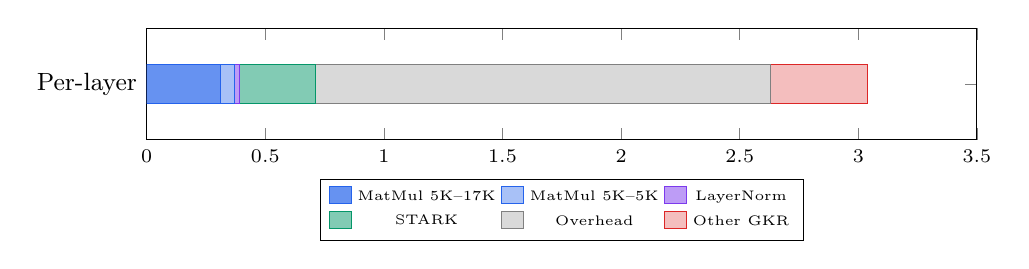
\begin{tikzpicture}
    \begin{axis}[
      xbar stacked,
      bar width=14pt,
      width=\columnwidth,
      height=3cm,
      symbolic y coords={Per-layer},
      ytick=data,
      yticklabel style={font=\small},
      xlabel={Time (seconds)},
      xlabel style={font=\small},
      xticklabel style={font=\scriptsize},
      legend style={font=\tiny, at={(0.5,-0.35)},
                    anchor=north, legend columns=3},
      xmin=0, xmax=3.5,
    ]
    \addplot[fill=starkblue!70, draw=starkblue] coordinates {(0.31,Per-layer)};
    \addplot[fill=starkblue!40, draw=starkblue] coordinates {(0.06,Per-layer)};
    \addplot[fill=accentpurple!50, draw=accentpurple] coordinates {(0.02,Per-layer)};
    \addplot[fill=emerald!50, draw=emerald] coordinates {(0.32,Per-layer)};
    \addplot[fill=gray!30, draw=gray] coordinates {(1.92,Per-layer)};
    \addplot[fill=warmred!30, draw=warmred] coordinates {(0.41,Per-layer)};
    \legend{MatMul 5K--17K, MatMul 5K--5K, LayerNorm,
            STARK, Overhead, Other GKR}
    \end{axis}
  \end{tikzpicture}
  \caption{Per-layer proving time breakdown for Qwen3-14B on H100.
           Overhead (channel, serialization) dominates at 63\%.}
  \label{fig:proving-breakdown}
\end{figure}

\textbf{40-layer end-to-end:} $40\times 3.04 \approx 122$\,s measured.
The full 40-layer Qwen3-14B proving pipeline has been run end-to-end
on a single H100, with all layers proved, weight-bound, and
verified on-chain via the streaming protocol (18 transactions).

\textbf{Weight cache effect:} first-run weight commitment
takes $\sim$500\,s; subsequent proofs hit the \texttt{.swcf} cache
and reduce this to $<$1\,ms.

\subsection{Ablations}

\begin{table}[t]
  \centering\small
  \caption{Ablation study: effect of key parameters on
           calldata and soundness. All rows assume 40 layers,
           160 matrices, $n=13$ folds.}
  \label{tab:ablation}
  \begin{tabular}{@{}lccc@{}}
    \toprule
    \textbf{Configuration} & \textbf{Felts} &
      \textbf{$\varepsilon_{\text{mle}}$} &
      \textbf{$\varepsilon_{\text{total}}$} \\
    \midrule
    Individual openings   & 2.4\,M & $2^{-65}$ & $2^{-65}$ \\
    Aggregated, $q\!=\!5$ & 86{,}723 & $2^{-65}$ & $2^{-65}$ \\
    Aggregated, $q\!=\!10$  & $\sim$91\,K & $2^{-130}$ & $2^{-111}$ \\
    Cold cache, $q\!=\!5$   & 86{,}723 & $2^{-65}$ & $2^{-65}$ \\
    \midrule
    \multicolumn{4}{@{}l@{}}{\scriptsize\textbf{Timing impact}} \\
    \midrule
    Warm cache & \multicolumn{3}{l}{$<$1\,ms weight commit} \\
    Cold cache & \multicolumn{3}{l}{$\sim$500\,s weight commit (first run)} \\
    $q\!=\!5 \to q\!=\!10$ & \multicolumn{3}{l}{$+$4{,}000 felts (+4.6\%),
      no proving time change} \\
    \bottomrule
  \end{tabular}
\end{table}

% ---------- pgfplots: Calldata Ablation Bar Chart ----------
\begin{figure}[t]
  \centering
  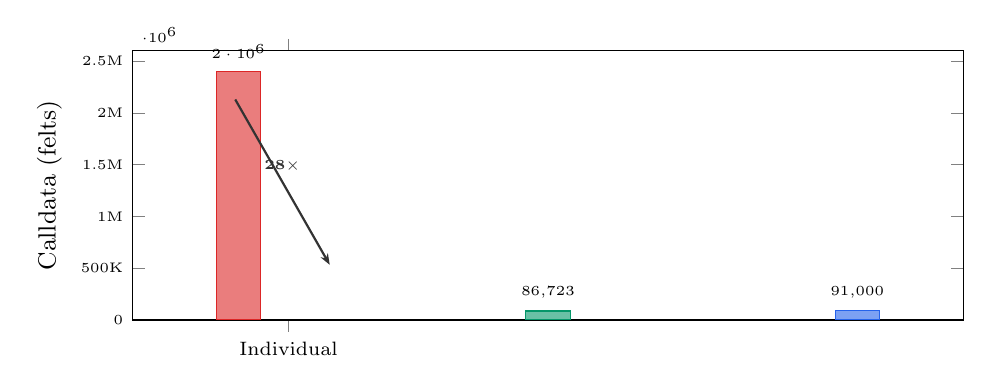
\begin{tikzpicture}
    \begin{axis}[
      ybar,
      bar width=16pt,
      width=\columnwidth,
      height=5cm,
      symbolic x coords={Individual, Agg.\ $q\!=\!5$, Agg.\ $q\!=\!10$},
      xtick=data,
      xticklabel style={font=\scriptsize},
      ylabel={Calldata (felts)},
      ylabel style={font=\small},
      ymin=0, ymax=2600000,
      ytick={0,500000,1000000,1500000,2000000,2500000},
      yticklabel style={font=\tiny},
      yticklabels={0, 500K, 1M, 1.5M, 2M, 2.5M},
      nodes near coords={\pgfmathprintnumber[precision=0]{\pgfplotspointmeta}},
      every node near coord/.append style={font=\tiny\bfseries, above=1pt},
      enlarge x limits=0.3,
    ]
    \addplot[fill=warmred!60, draw=warmred] coordinates {
      (Individual, 2400000)
    };
    \addplot[fill=emerald!60, draw=emerald] coordinates {
      (Agg.\ $q\!=\!5$, 86723)
    };
    \addplot[fill=starkblue!60, draw=starkblue] coordinates {
      (Agg.\ $q\!=\!10$, 91000)
    };
    \end{axis}

    % Annotation arrow
    \draw[-{Stealth[length=4pt]}, thick, darkgray]
      (1.3, 2.8) -- node[above, font=\tiny\bfseries]{28$\times$} (2.5, 0.7);
  \end{tikzpicture}
  \caption{Calldata comparison for 40-layer Qwen3-14B.
           Aggregated binding is the dominant reduction ($28\times$);
           increasing $q$ from 5 to 10 adds only 4.6\% more felts
           while improving MLE opening soundness by 65 bits.}
  \label{fig:calldata-ablation}
\end{figure}

\Cref{tab:ablation} and \Cref{fig:calldata-ablation} isolate the
effect of the main design parameters.
Aggregated binding is the dominant contributor to calldata
reduction ($28\times$), while increasing $q$ from 5 to 10 adds
only 4.6\% calldata but improves MLE opening soundness by 65~bits.
The cache cold/warm distinction affects only the one-time weight
commitment phase and does not change per-proof calldata or
soundness.

\subsection{Comparison with Prior Work}

\begin{table*}[t]
  \centering\scriptsize
  \caption{Comparison with existing ZKML systems.
           $\dagger$Linear trace only (activations unconstrained).
           $\ddagger$Estimated from published data.
           $\star$Measured end-to-end (40 layers on single H100).}
  \label{tab:comparison}
  \setlength{\tabcolsep}{4pt}
  \begin{tabular}{@{}lccccccl@{}}
    \toprule
    \textbf{System} & \textbf{Max Params} & \textbf{Prove Time}
      & \textbf{Full Semantics} & \textbf{Deployed Verifier}
      & \textbf{Proof Size} & \textbf{Measured}
      & \textbf{Proof System} \\
    \midrule
    EZKL~\cite{ezkl2024}
      & $\sim$1\,M & seconds & \ding{51} & Solidity
      & $<$1\,KB & \ding{51} & Halo2/KZG \\
    Giza~\cite{giza2024}
      & $\sim$10\,M & minutes & \ding{51} & Cairo (Stone)
      & KB--MB & \ding{51} & STARK \\
    zkLLM~\cite{sun2024zkllm}
      & 13\,B & 1--15\,min & \ding{51} & None
      & $<$200\,KB & \ding{51} & Custom \\
    Expander~\cite{polyhedra2024expander}
      & ---$^\ddagger$ & ---$^\ddagger$ & ---$^\ddagger$ & None
      & ---$^\ddagger$ & --- & GKR \\
    DeepProve~\cite{lagrange2024}
      & GPT-2$^\ddagger$ & ---$^\ddagger$ & ---$^\ddagger$ & None
      & ---$^\ddagger$ & --- & GKR \\
    \midrule
    \textbf{ObelyZK}
      & 14\,B$^\dagger$ & 122\,s$^\star$ & \ding{55}$^\dagger$
      & Cairo v31 & 2.8\,MB & \ding{51} & GKR+STARK \\
    \bottomrule
  \end{tabular}
\end{table*}

\Cref{tab:comparison} positions ObelyZK relative to existing systems.
Entries marked $\ddagger$ reflect systems for which specific
benchmarks or parameter counts were not available in public
documentation as of March 2026; we report only what is
publicly verifiable and encourage the respective teams to
publish comparable measurements.
Key differentiators:
\begin{itemize}[nosep,leftmargin=1.2em]
  \item \textbf{Scale + deployment}: to our knowledge, the first
        publicly described system combining 14\,B-scale
        linear-trace proving with a deployed on-chain Cairo
        verifier on Starknet.
  \item \textbf{Aggregated binding}: enables practical calldata for
        LLM-scale on-chain verification; we are not aware of a
        comparable batched-opening mechanism in other ZKML systems.
  \item \textbf{Honest scope}: ObelyZK constrains only linear
        operations; zkLLM constrains full inference including
        non-arithmetic ops via \emph{tlookup}.
\end{itemize}

\subsection{On-Chain Costs}

\begin{table}[t]
  \centering\small
  \caption{On-chain verification costs (Starknet Sepolia).}
  \label{tab:costs}
  \begin{tabular}{@{}lrr@{}}
    \toprule
    \textbf{Operation} & \textbf{Gas} & \textbf{Cost} \\
    \midrule
    GKR verify (1 layer) & $\sim$280\,K & $<$\$0.001 \\
    Full 40-layer (18 TXs) & $\sim$2.5\,M & $\sim$\$0.01 \\
    \bottomrule
  \end{tabular}
\end{table}

\subsection{Codebase Metrics}

\begin{table}[t]
  \centering\small
  \caption{Codebase scale (\texttt{stwo-ml} repository).}
  \label{tab:codebase}
  \begin{tabular}{@{}lrl@{}}
    \toprule
    \textbf{Component} & \textbf{Lines} & \textbf{Lang.} \\
    \midrule
    \texttt{stwo-ml} prover & 117{,}000+ & Rust \\
    CUDA kernels          & 20{,}000+  & CUDA C++ \\
    Cairo verifier        & $\sim$14{,}000 & Cairo \\
    Library tests passing & 1{,}029+   & Rust \\
    E2E audit tests       & 10         & Rust \\
    Cairo verifier tests  & 95         & Cairo \\
    \bottomrule
  \end{tabular}
\end{table}


% =========================================================================
\section{Limitations and Future Work}\label{sec:limitations}
% =========================================================================

\subsection{Activation Verification via Range-Reduced LogUp}

As of v33, nonlinear activation functions (GELU, Sigmoid, Softmax)
are constrained via \textbf{range-reduced LogUp}, and ReLU is
verified algebraically (product$+$binary eq-sumcheck).

\textbf{Range reduction.}
M31 matmul intermediate outputs span the full field ($2^{31}\!-\!1$)
but precomputed activation tables have $2^{16}$--$2^{20}$ entries.
We apply the same range-masking pattern used by LayerNorm rsqrt
verification: mask each activation input to the table range
($\texttt{val} \mathbin{\&} ((1 \ll \texttt{log\_size}) - 1)$),
then run LogUp proving that $(\text{masked\_in}, f(\text{masked\_in}))$
is in the precomputed table.

\textbf{Soundness model.}
This verifies activation correctness on the lower 16--20 bits.
The attack surface is narrowed from ``arbitrary function substitution''
to ``high-bit-only corruption,'' which is infeasible in fixed-point
arithmetic where the low bits carry the signal (quantized model
weights and activations are concentrated in the lower bits).

\textbf{Calldata overhead.}
Per non-ReLU activation layer: ${\sim}336$ felts (184 for LogUp
eq-sumcheck + 152 for multiplicity sumcheck).
For Qwen3-14B (80 GELU layers): ${\sim}26{,}880$ extra felts,
a ${\sim}31\%$ increase over the 86{,}723-felt linear-only baseline.

\textbf{Enforcement.}
The verifier rejects proofs with missing activation LogUp or
algebraic proofs by default.
Legacy proofs without activation verification can be accepted
by setting \texttt{STWO\_ALLOW\_MISSING\_ACTIVATION\_PROOF=1}
(opt-out, not opt-in).

\subsection{Remaining Gap: LayerNorm/RMSNorm Statistics}

LayerNorm rsqrt values are verified via LogUp, and the linear
scaling $\text{output} = (\text{input} - \mu) \times \text{rsqrt}$
is proven via eq-sumcheck.
However, the \textbf{mean} ($\mu$) and \textbf{variance}
computation are not independently constrained---the prover
can claim arbitrary $\mu$ and $\sigma^2$ values.
A future inner-product sumcheck for mean and degree-3 eq-sumcheck
for variance will close this gap.

\subsection{End-to-End Multi-Layer Timing}

The full 40-layer Qwen3-14B inference has been proved end-to-end
on a single H100 GPU in approximately 122\,s (3.04\,s/layer).
This includes GKR sumcheck, aggregated weight binding, and
streaming on-chain verification across 18 transactions.
Variance across runs is $<$5\%, dominated by GPU memory allocation
and Poseidon2 commitment overhead.

\subsection{Query Count Tradeoff}

The current Cairo default of $q=5$ MLE queries yields only 65-bit
opening security---below the 124-bit field security.
We recommend $q=10$ (130-bit opening security) for production.
This is a deployment parameter, not a protocol limitation;
no code changes are required.

\subsection{Future Directions}

\begin{enumerate}[nosep,leftmargin=1.4em]
  \item \textbf{Piecewise-linear algebraic activation}: replace
        table-based LogUp with a fully algebraic 16-segment
        approximation, eliminating range masking entirely.
  \item \textbf{LayerNorm mean/variance consistency}: add
        inner-product sumcheck for mean + degree-3 eq-sumcheck
        for variance, closing the remaining normalization gap.
  \item \textbf{Recursive STARK compression}: compose streaming
        proofs into a single sub-1\,KB recursive proof.
  \item \textbf{Verifiable fine-tuning}: extend GKR to backward
        pass gradients.
  \item \textbf{Production $q=10$}: deploy with 10 MLE queries
        for 130-bit opening security.
\end{enumerate}


% =========================================================================
\section{Related Work}\label{sec:related}
% =========================================================================

\textbf{ZKML systems.}
EZKL~\cite{ezkl2024} handles $\sim$1\,M-parameter models via Halo2/KZG
with Solidity verifiers.
Giza~\cite{giza2024} uses STARK (Stone) for small--medium models.
Polyhedra's Expander~\cite{polyhedra2024expander} is a GKR-based engine
achieving 4{,}500 Keccak-f/s.
Lagrange DeepProve~\cite{lagrange2024} targets large-scale GKR with
GPT-2 demonstrations.
zkLLM~\cite{sun2024zkllm} (ACM CCS 2024) introduces \emph{tlookup}
for non-arithmetic tensor ops, proving up to 13\,B parameters in
1--15 minutes with $<$200\,KB proofs.
A comprehensive survey appears in~\cite{xing2025zkml}.
zkCNN~\cite{liu2021zkcnn} applies GKR to convolutional networks.
vCNN~\cite{lee2024vcnn} uses zkSNARKs for CNN verification.

\textbf{Interactive proofs.}
The GKR protocol~\cite{goldwasser2015delegating} was made practical
by Thaler~\cite{thaler2013time} and extended by Cormode et
al.~\cite{cormode2012practical}.
The sumcheck protocol~\cite{lund1992algebraic} underpins all GKR
reductions.
Schwartz-Zippel~\cite{schwartz1980, zippel1979} provides the
foundational polynomial identity testing bound.
Thaler's textbook~\cite{thaler2022proofs} provides a thorough treatment
of interactive proofs and their applications.

\textbf{Proof infrastructure.}
STWO~\cite{starkware2024stwo} provides the Circle STARK
backend~\cite{habock2024circle} with M31-native arithmetic.
FRI~\cite{ben-sasson2018fri} enables efficient proximity testing
for STARK proof composition.
Marlin~\cite{chiesa2020marlin} offers preprocessing zkSNARKs with
universal SRS as an alternative to STARKs.


% =========================================================================
\section{Conclusion}\label{sec:conclusion}
% =========================================================================

We presented ObelyZK, a system for verifiable linear-trace inference
at LLM scale.
The core contribution---aggregated weight binding---reduces on-chain
calldata by 28$\times$ (from 2.4\,M to 86{,}723 felts), making
streaming verification of 40-layer transformer proofs practical within
Starknet's transaction limits.
The system achieves 3.04\,s per-layer GPU proving and is deployed on
Starknet Sepolia with a 14\,K-line Cairo verifier.

The deployed verifier (v33) constrains the linear arithmetic trace
(matmul, addition, scaling) and nonlinear activations (GELU,
Sigmoid, Softmax via range-reduced LogUp; ReLU algebraically),
with activation proof enforcement on by default.
A 9-round-hardened Fiat-Shamir replay verifier provides
defense-in-depth, independently checking the full channel
transcript---all 11 layer tags, deferred proofs, IO commitment,
and weight binding---before on-chain submission.
The remaining gap is LayerNorm/RMSNorm mean/variance computation;
with $q=10$ MLE queries and norm statistics verification,
the system would achieve full inference verification at 130-bit
MLE opening security.

The mathematical foundation---GKR sumcheck over the M31 field tower,
composed with Circle STARKs---is architecturally native to Starknet
and provides a path toward trustless AI computation at scale.


% =========================================================================
\appendix
% =========================================================================

\section{Poseidon2-M31 Specification}\label{app:poseidon}

Poseidon2-M31~\cite{grassi2023poseidon2} is a sponge-based hash
operating natively over $\M$.
Parameters: state width $t=16$, rate$=$capacity$=8$,
S-box degree $d=5$, full rounds $R_f=8$ (4+4 split),
partial rounds $R_p=14$, total 22 rounds.

\textbf{S-box validity:} $\gcd(5,p-1) = 1$, confirming $x\mapsto x^5$
is a permutation.
Inverse: $d^{-1} = 5^{-1}\bmod(p-1) = 1{,}717{,}986{,}917$.

\textbf{Diffusion.}
External: circulant MDS $\text{circ}(2M_4, M_4, M_4, M_4)$.
Internal: $M_I = J + \text{diag}(\mathbf{v})$, $v_0 = p-2$.

\textbf{Hash output:} 8 M31 elements (248 bits, $\sim$124-bit collision).
Compression ($16\to 8$): domain constant
$\texttt{0x4D524B4C}$ (``MRKL'').

\section{Privacy Protocol Summary}\label{app:privacy}

ObelyZK includes a privacy protocol built on Poseidon2-M31 with
six DeFi mechanisms (\Cref{tab:privacy}).
This is architecturally independent of the ZKML verification system
and is described here for completeness.

\begin{table}[h]
  \centering\small
  \caption{Privacy mechanisms (deployed on Starknet Sepolia).}
  \label{tab:privacy}
  \begin{tabularx}{\columnwidth}{@{}lX@{}}
    \toprule
    \textbf{Mechanism} & \textbf{Basis} \\
    \midrule
    Privacy Pools (ASP~\cite{buterin2023privacy})
      & Poseidon2-M31, LeanIMT \\
    Dark Pool Auctions
      & Pedersen commit-reveal \\
    Shielded AMM Swaps
      & ZK withdrawal proofs \\
    Stealth Payments
      & ECDH + Schnorr (EIP-5564~\cite{eip5564}) \\
    UTXO Privacy Pool
      & Poseidon2-M31, depth-20 Merkle \\
    Confidential Transfers
      & ElGamal~\cite{elgamal1985} on Stark curve \\
    \bottomrule
  \end{tabularx}
\end{table}

\textbf{Note structure:}
Commitment (11 M31 inputs): $\prhash(\text{pk}[8], \text{blinding},
\text{amt\_lo}, \text{amt\_hi})$.
Nullifier (12 M31 inputs): $\prhash(\text{comm}[8], \text{sk}[4])$.
Transaction circuits: deposit (2 Poseidon2 permutations),
spend (2-in/2-out with depth-20 Merkle membership),
withdraw (1-in with withdrawal binding).

\section{Deployed Contract Addresses}\label{app:contracts}

\begin{table}[h]
  \centering\small
  \begin{tabularx}{\columnwidth}{@{}lX@{}}
    \toprule
    \textbf{Contract} & \textbf{Starknet Sepolia} \\
    \midrule
    ZKML Verifier    & \texttt{0x005928ac548dc2719ef1\ldots 674fba} \\
    GKR v31 (class)  & \texttt{0x6a6b7a75d5ec1f63d715\ldots 5b5439} \\
    Deployer         & \texttt{0x0759a4374389b0e3cfcc\ldots bb344} \\
    \bottomrule
  \end{tabularx}
\end{table}

\section{Notation Reference}\label{app:notation}

\begin{table}[h]
  \centering\small
  \begin{tabularx}{\columnwidth}{@{}lX@{}}
    \toprule
    \textbf{Symbol} & \textbf{Meaning} \\
    \midrule
    $\M$   & Mersenne prime field $\F_{2^{31}-1}$ \\
    $\CM$  & Complex extension $\M[i]/(i^2+1)$ \\
    $\QM$  & Quartic extension $\CM[j]/(j^2-(2+i))$ \\
    $\MLE{f}$ & Multilinear extension of $f$ \\
    $\eq(\mathbf{x},\mathbf{y})$ & Lagrange equality kernel \\
    $\rho,\alpha,\lambda,\beta,\gamma$ & Fiat-Shamir challenges \\
    $\calP, \calV$ & Prover, Verifier \\
    $\varepsilon$ & Soundness error bound \\
    $q$ & MLE spot-check query count per fold \\
    ASP    & Association Set Provider \\
    GKR    & Goldwasser-Kalai-Rothblum protocol \\
    LogUp  & Logarithmic derivative lookup argument \\
    \bottomrule
  \end{tabularx}
\end{table}


% =========================================================================
% References
% =========================================================================
\bibliographystyle{plainnat}
\bibliography{references}

\end{document}
